\begin{figure}[hbt!]
    \centering
    \begin{tikzpicture}
    \node[anchor=south west,inner sep=0] (image) at (0,0) {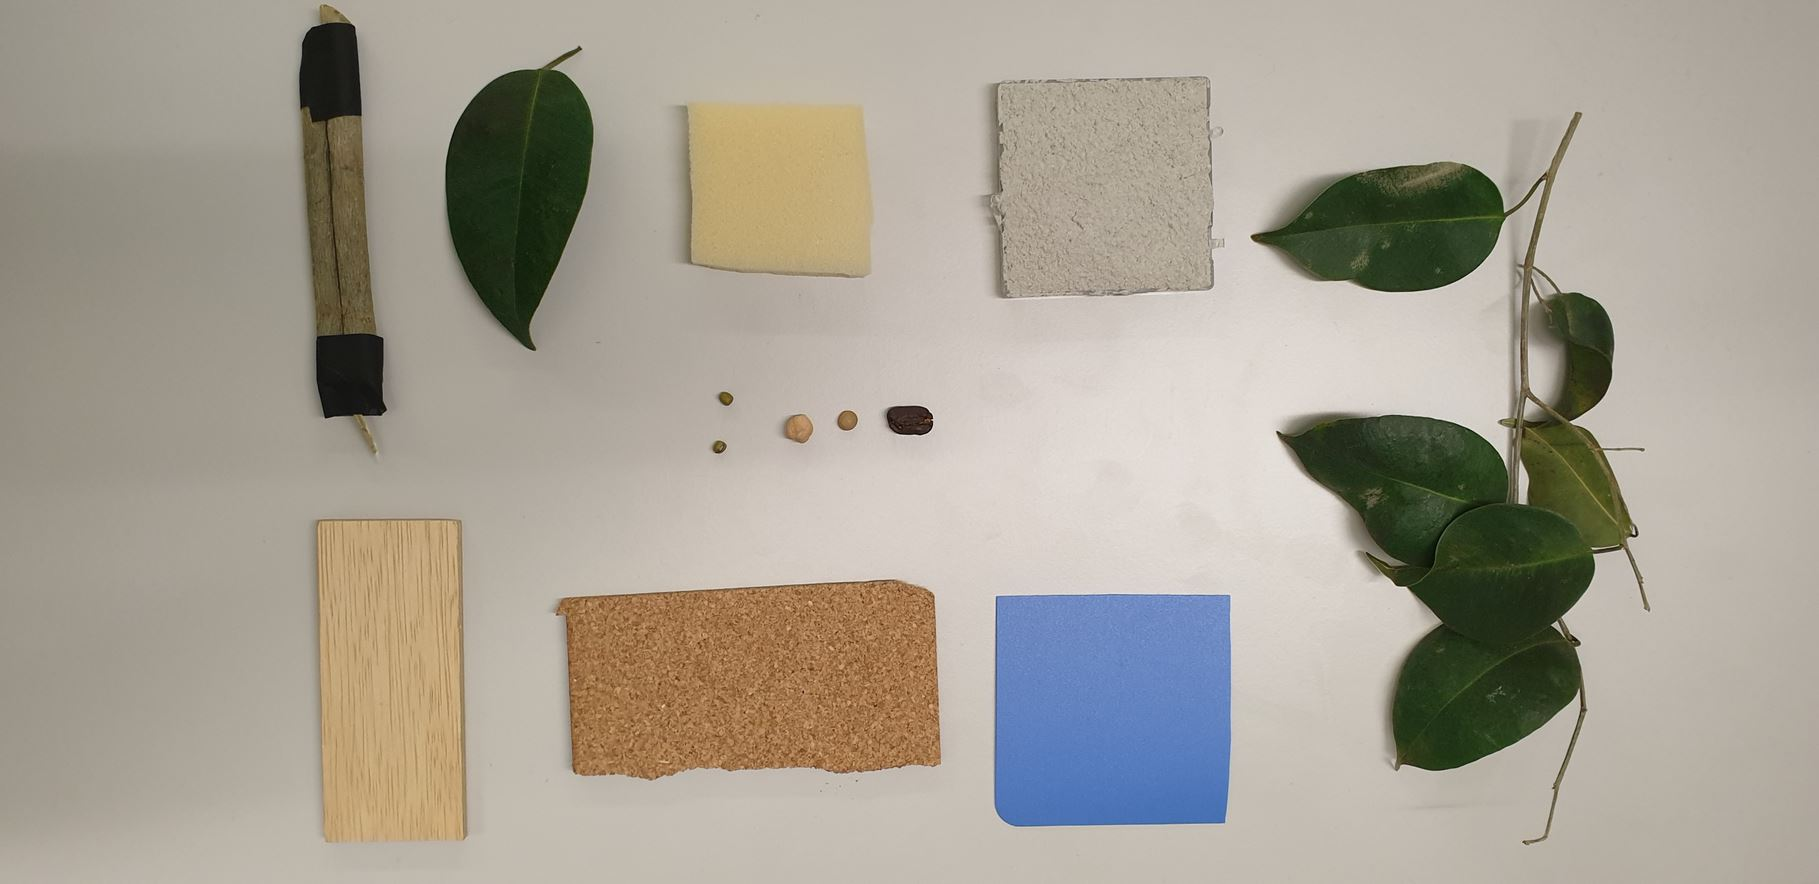
\includegraphics[width=0.9\textwidth]{chapters/papers/ED/resources/images/multi-spectral/material_samples.png}};
    \begin{scope}[x={(image.south east)},y={(image.north west)}]
        \node [rounded corners, fill=white] at (0.18, 0.92) {branch};
        \node [rounded corners, fill=white] at (0.29, 0.92) {leaf};
        \node [rounded corners, fill=white] at (0.42, 0.92) {foam};
        \node [rounded corners, fill=white] at (0.6, 0.92) {plaster};
        \node [rounded corners, fill=white] at (0.21, 0.38) {wood};
        \node [rounded corners, fill=white] at (0.42, 0.38) {cork};
        \node [rounded corners, fill=white] at (0.6, 0.38) {plastic};
    \end{scope}
    \end{tikzpicture}%
    \imageTable{resources/plots/multi-spectral}{individual-curves}{/}{branch, leaf, foam}{}{}{.011\textwidth}{.011\textwidth}
    \caption{We evaluate the multi-spectral imaging capabilities using a number of material samples. The resulting intensity measurements are normalized and compared to readings from a ground-truth spectrometer reading and a commercial camera system (MicaSense RedEdge-MX Dual).}
    \label{fig:materialResponses}
\end{figure}